\documentclass[10pt]{article}
\usepackage{pgfplots}
\usepackage{physics}
\usepackage{tikz}
\pgfplotsset{compat=1.15}
\usepackage{mathrsfs}
\usetikzlibrary{arrows}
\pagestyle{empty}
\begin{document}

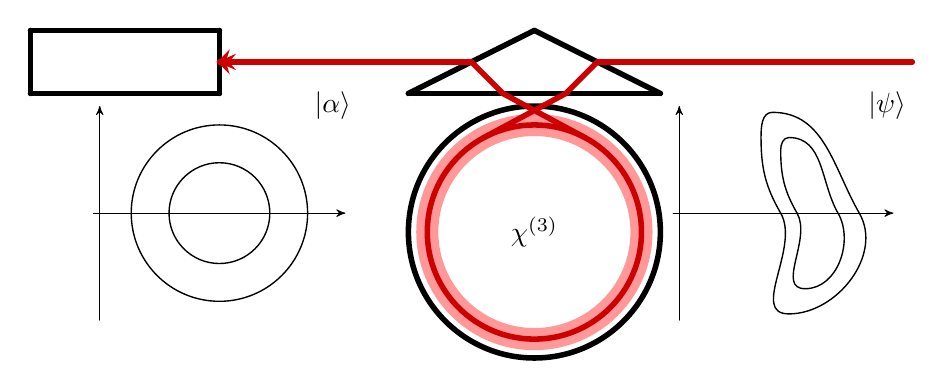
\begin{tikzpicture}[line cap=round,line join=round,>=triangle 45,x=1cm,y=1cm, 
    axis/.style={line width= 0.3pt, ->, >=stealth'}, scale=0.8]
% \clip(-5.208032545829854,-6.506121870314113) rectangle (15.714449254128738,6.275612465660563);
\definecolor{ccqqqq}{rgb}{0.8,0,0}
\definecolor{lightred}{rgb}{1,0.6,0.6}
\def\scal{0.65}

% rect
\draw [line width=2pt] (0,0) -- (3,0);
\draw [line width=2pt] (3,1) -- (3,0);
\draw [line width=2pt] (3,1) -- (0,1);
\draw [line width=2pt] (0,1) -- (0,0);
% triang
\def\lev{0.5}
\def\v{0.5}
\draw [line width=2pt] (6,\lev-\v)-- (10,\lev-\v);
\draw [line width=2pt] (8,\lev+\v)-- (10,\lev-\v);
\draw [line width=2pt] (8,\lev+\v)-- (6,\lev-\v);
% horisontal laser
\draw [line width=2pt,color=ccqqqq] (3,\lev) -- (7,\lev);
\draw [line width=2pt,color=ccqqqq] (9,\lev) -- (14,\lev);
% nonhorizontal in triangle
\draw [line width=2pt,color=ccqqqq] (7,\lev) -- (7.5,\lev-\v);
\draw [line width=2pt,color=ccqqqq] (9,\lev) -- (8.5,\lev-\v);
% resonator
\def\centy{\lev-2.7}
\draw [line width=2pt] (8,\centy) circle (2);
% lines in resonator
% circle
\draw [line width=8pt,color=lightred] (8,\centy) circle (1.7);
\draw [line width=2pt,color=ccqqqq] (8,\centy) circle (1.7);
% tangent line
\draw [line width=2pt,color=ccqqqq] (7.5,\lev-\v) -- (8.805956084154726, -0.7031917990557444);
\draw [line width=2pt,color=ccqqqq] (8.5,\lev-\v) -- (7.194043915845274, -0.7031917990557441);
% laser
\fill [ccqqqq] (3cm - 1pt,\lev) -- ++(0.2, 0.2) -- (3+0.1,\lev);
\fill [ccqqqq] (3cm - 1pt,\lev) -- ++(+0.2, -0.2) -- (3+0.1,\lev);
\fill [ccqqqq] (3cm - 1pt,\lev) -- ++(0.3, 0.13) -- (3+0.15,\lev);
\fill [ccqqqq] (3cm - 1pt,\lev) -- ++(+0.3, -0.13) -- (3+0.15,\lev);
% TEXT
\def\s{4}
\def\sh{-0.6}
\def\h{1.7}
% chi (3)
\node[] at (5-.2,\lev +\sh*\s+\h) {$\ket{\alpha}$};
\node[] at (10.3+3.3,\lev +\sh*\s+\h) {$\ket{\psi}$};
\node[align=center] at (8,\centy) {$\chi^{(3)}$};
% Axis
\draw[axis] (1, \lev +\sh*\s) -- (5, \lev +\sh*\s) node(xline)[right]{};
\draw[axis] (1.1, \lev +\sh*\s - \h) -- (1.1, \lev +\sh*\s+\h) node(yline)[above] {};
\draw[axis] (10.2, \lev +\sh*\s) -- (10.2+3.5, \lev +\sh*\s) node(xline)[right]{};
\draw[axis] (10.3, \lev +\sh*\s - \h) -- (10.3, \lev +\sh*\s + \h) node(yline)[above] {};
% Plot circles
\draw [line width=0.5pt] (3,\lev +\sh*\s) circle (0.35*\s);
\draw [line width=0.5pt] (3,\lev +\sh*\s) circle (0.2*\s);
% Plot curves 10.3+1.9 = 12.1
\def\ssh{0.3}
\draw[line width=0.5pt] (5+7+\ssh+0.2*\scal * \s, \lev +\sh * \s) to [out=120, in=0] ++(-0.3*\scal*\s, + 0.3*\s)
    to [out=180, in=90] ++ (-0.05*\scal*\s, -0.05*\s)
    to [out=270, in=120] (5+7+\ssh-0.05*\scal*\s, \lev +\sh*\s)
    to [out=300, in=180] (5+7+\ssh, \lev+\sh*\s - 0.3*\s)
    to [out=0, in=300] (5+7+\ssh+0.2*\scal*\s, \lev +\sh*\s);
\draw[line width=0.5pt] (5+7+\ssh+0.33*\scal*\s, \lev +\sh*\s) to [out=120, in=0] ++(-0.33*\scal*\s - 0.2*\scal*\s, + 0.4*\s)
    to [out=180, in=90] ++ (-0.07*\scal*\s, -0.1*\s)
    to [out=270, in=120] (5+7+\ssh-0.15*\scal*\s, \lev +\sh*\s)
    to [out=300, in=180] (5+7+\ssh-0.1*\scal*\s, \lev+\sh*\s - 0.4*\s)
    to [out=0, in=300] (5+7+\ssh+0.33*\scal*\s, \lev +\sh*\s);
\end{tikzpicture}
\end{document}